
%---------------------------------------------------------------
% The "*" following chapter or section commands omits chapter/
% section numbers.  It also does not include the chapter/section
% in the table of contents -- the \addcontentsline can be used
% to manually force its entry.
%---------------------------------------------------------------

\chapter*{Introduction}
\addcontentsline{toc}{chapter}{Introduction}

The continued reduction of the transistor feature size has led to the increase in the vulnerability of modern circuits to error. This effect, in turn, has made modern circuits more susceptible to radiation induced errors in space and terrestrial environments. A radiation induced error, commonly referred to as a soft error, occurs when a high energy particle from space or packaging strikes a transistor. Shown in Fig. \ref{strike}, the particle deposits energy in the active volume generating electron-hole pairs. This creates a new diffusion region that could allow a non-conducting device to temporarily conduct current. The mechanism causes a temporary voltage pulse, referred to as a single event transient (SET) to occur at the device.

\begin{figure}[!htbp]
	\centering
	
\includegraphics[width=0.45\linewidth]{Figures/StrikeFig}
	%where an .eps filename suffix will be assumed under latex, 
	%and a .pdf suffix will be assumed for pdflatex; or what has been declared
	%via \DeclareGraphicsExtensions.
	\caption{A energetic particle creating electron-hole pairs in a transistor.}
	\label{strike}
\end{figure} 

In the case of a radiation particle striking a memory storage element, the data stored in the device can be changed. If the device loses its value due to a strike by a single particle, this is referred to as a single event upset (SEU). Additionally, due to the constant scaling down of the feature size, a single particle can also strike two transistors simultaneously which is referred to as a double node upset (DNU). Fig. \ref{DNUStrike} gives a diagram of a SEU tolerant latch to demonstrate the DNU phenomenon. In the diagram, radiation is denoted as a high energy particle which passes through two transistors on a DICE latch \cite{DICE}. In the case of a SEU, the DICE latch would normally be able to tolerate the error. As can be observed, the particle passes through two transistors causing the respective node to switch from "1" on the first node to "0" and from "0" to "1" on the second node. The upset of both nodes drives the remaining two nodes to an erroneous value. This observance is alarming since it signals that current designs are not sufficient for future processes. In turn, this provides a need for new memory element designs that can tolerate DNUs. 

\begin{figure}[!htbp]
	\centering
	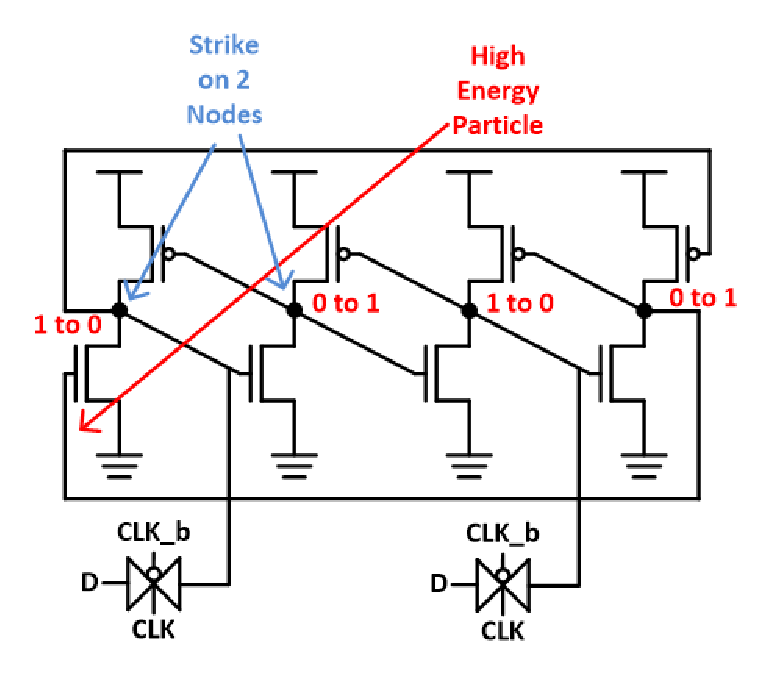
\includegraphics[width=0.45\linewidth]{Figures/StrikeonDICE}
	%where an .eps filename suffix will be assumed under latex, 
	%and a .pdf suffix will be assumed for pdflatex; or what has been declared
	%via \DeclareGraphicsExtensions.
	\caption{A particle striking two node concurrently causing a double node upset.}
	\label{DNUStrike}
\end{figure} 

Additionally, modern circuit designs employ a technique referred to as clock gating. Clock gating is defined as setting the clock to constant value thus reducing the power consumed. Use of clock gating may lead to cases where the current state held by the memory element must be held for many clock cycles. This need leads to a much longer than normal vulnerable window in which an improperly hardened device may lose the stored value. While there are existing DNU tolerant designs \cite{Inter,DNCS,HSMUF}, these designs move to a high impedance state after a DNU. If a DNU occurs while the latch is gated, the voltages within the latch may degrade. In Chapter 1, we aim to alleviate this problem by providing an efficient design that is capable of recovering all nodes after a DNU occurs. This, in effect, guarantees that the data will be held even if the latch is struck by a DNU while gated.

In addition to the effects on memory elements, accurate approximation of the error rate of a circuit is also important. The goal of circuit simulation is the accurate estimation of the soft error rate (SER). In this work, the focus is on the evaluation of combinational circuits. Typically, this type of simulation entails the estimation of the resulting pulse shape when a particle strike a transistor, the determination of the boolean functions that allow the pulse to propagate and the estimation of the latching characteristics at an output flip-flop. Using these parameters, the probability of the pulse reaching an output flip-flop is determined. Assume that the probability of an error reaching and being latched in a flip-flop at output \textit{i} of the circuit is represented as \textit{$P(O_i)$}, the particle hit rate in a particular area is given as \textit{$R_{PH}$}, the fraction of particle hits resulting in charge generation as \textit{$R_{eff}$} and \textit{$A_{cir}$} gives the area of the circuit. The equation for the SER at output \textit{$O_i$} is given below \cite{METSys}.

\begin{equation}\label{SER_eq}
SER_{O_i} = P(O_i) * R_{eff} * R_{PH} * A_{cir}
\end{equation}

The focus of all SER estimation simulators is the calculation of the term \textit{$P(O_i)$}. This is a difficult problem in combination circuits due to the presence of the following three masking factors: electrical masking, logical masking and temporal masking. Electrical masking deals with the calculation of the pulse shape as it propagates through the circuit. Logical masking is the estimation of the logical 1's and 0's and how they may mask the pulse. For example, if a NAND gate has a value of "0" on an input, the pulse will not propagate since the output will be held to a "1". Lastly, temporal masking involves the latching characteristics, specifically the set-up and hold times, of the output flip flop. Accurate consideration of all three masking effects is crucial to accurate SER estimation.

Accurate consideration of the electrical masking effect is an important but often simplified component of SER estimation. The most common method to calculate the pulse shape, proposed in \cite{Omana_Trap} uses a linear line to approximate the rising and falling transitions giving a trapezoidal shape. While this method executes quickly and is easy to implement, it does not provide an accurate estimation of the pulse shape. As can be observed in Fig. [ref], a transient pulse does not take a trapezoidal shape in a real case. For this reason, accurate consideration of the pulse shape must consider the non-linear aspects of the pulse. In \cite{Accurate_Masking}, the authors proposed an enhanced pulse approximation method which is accurate within 5\% of HSPICE. 